\documentclass{article}

\usepackage{graphicx}

\usepackage[utf8]{inputenc}
\usepackage[margin=1.25in]{geometry}

\begin{document}

% Title page
\begin{titlepage}
    \centering{
        \vspace*{2cm}
        \Huge{
        Core101: User Guide (draft) \\
        }
        \vspace{5cm}
        \Huge{
        L0G1Candes \\
        }
        \vspace{5cm}
        \large{
        Centro de Microelectrónica de la Universidad de Los Andes (CMUA) \\
        Universidad de Los Andes \\
        Bogotá D.C., Colombia \\
        }
        \vfill
        \large{
        December 2019
        }
    }
\end{titlepage}

\tableofcontents

\listoffigures

\listoftables

\newpage
\section{Introduction}
Core101 is a RISC-V core intended to be used in FPGAs as an academic resource. The main objective behind Core101 is having a fully open core emphasizing in hardware design. In order to achieve the intended hardware emphasis, hardware description is written in Verilog in such a way that allows a user to use it on an open-source FPGA like tinyFPGA-BX, and the Verilog code is not written in a behavioural fashion but in a modular style. At the same time, the microarchitecture is fully described in this document. Another goal that is desired with this core is using a real-time operating system (RTOS) along with an embedded system whose main core is Core101. SoC101, the name for the embedded system, will be developed as the core development is finished.

\subsection{Specifications}
Table \ref{tab:specs0} summarizes Core101 specifications. Since the project is continuously evolving, Table \ref{tab:specs0} contains specifications for the last stable release. Nevertheless, previous releases specifications can be found in Appendix A.

\begin{table}[h]
    \centering
    \begin{tabular}{|l|l|}
        \hline
        \textbf{Specification}  &   \textbf{Value}      \\  \hline
        ISA                     &   RISC-V              \\  \hline
        ISA specifications      &   I (integer)         \\  \hline
        Architecture            &   Modified Harvard    \\  \hline
        Memory width            &   64 bits             \\  \hline
        Pipeline stages         &   1                   \\  \hline
        Release date            &   December 16th, 2019 \\  \hline
        
    \end{tabular}
    \caption{Summary of Core101 specifications.}
    \label{tab:specs0}
\end{table}

\section{Microarchitecture}

\begin{figure}[h]
    \centering
    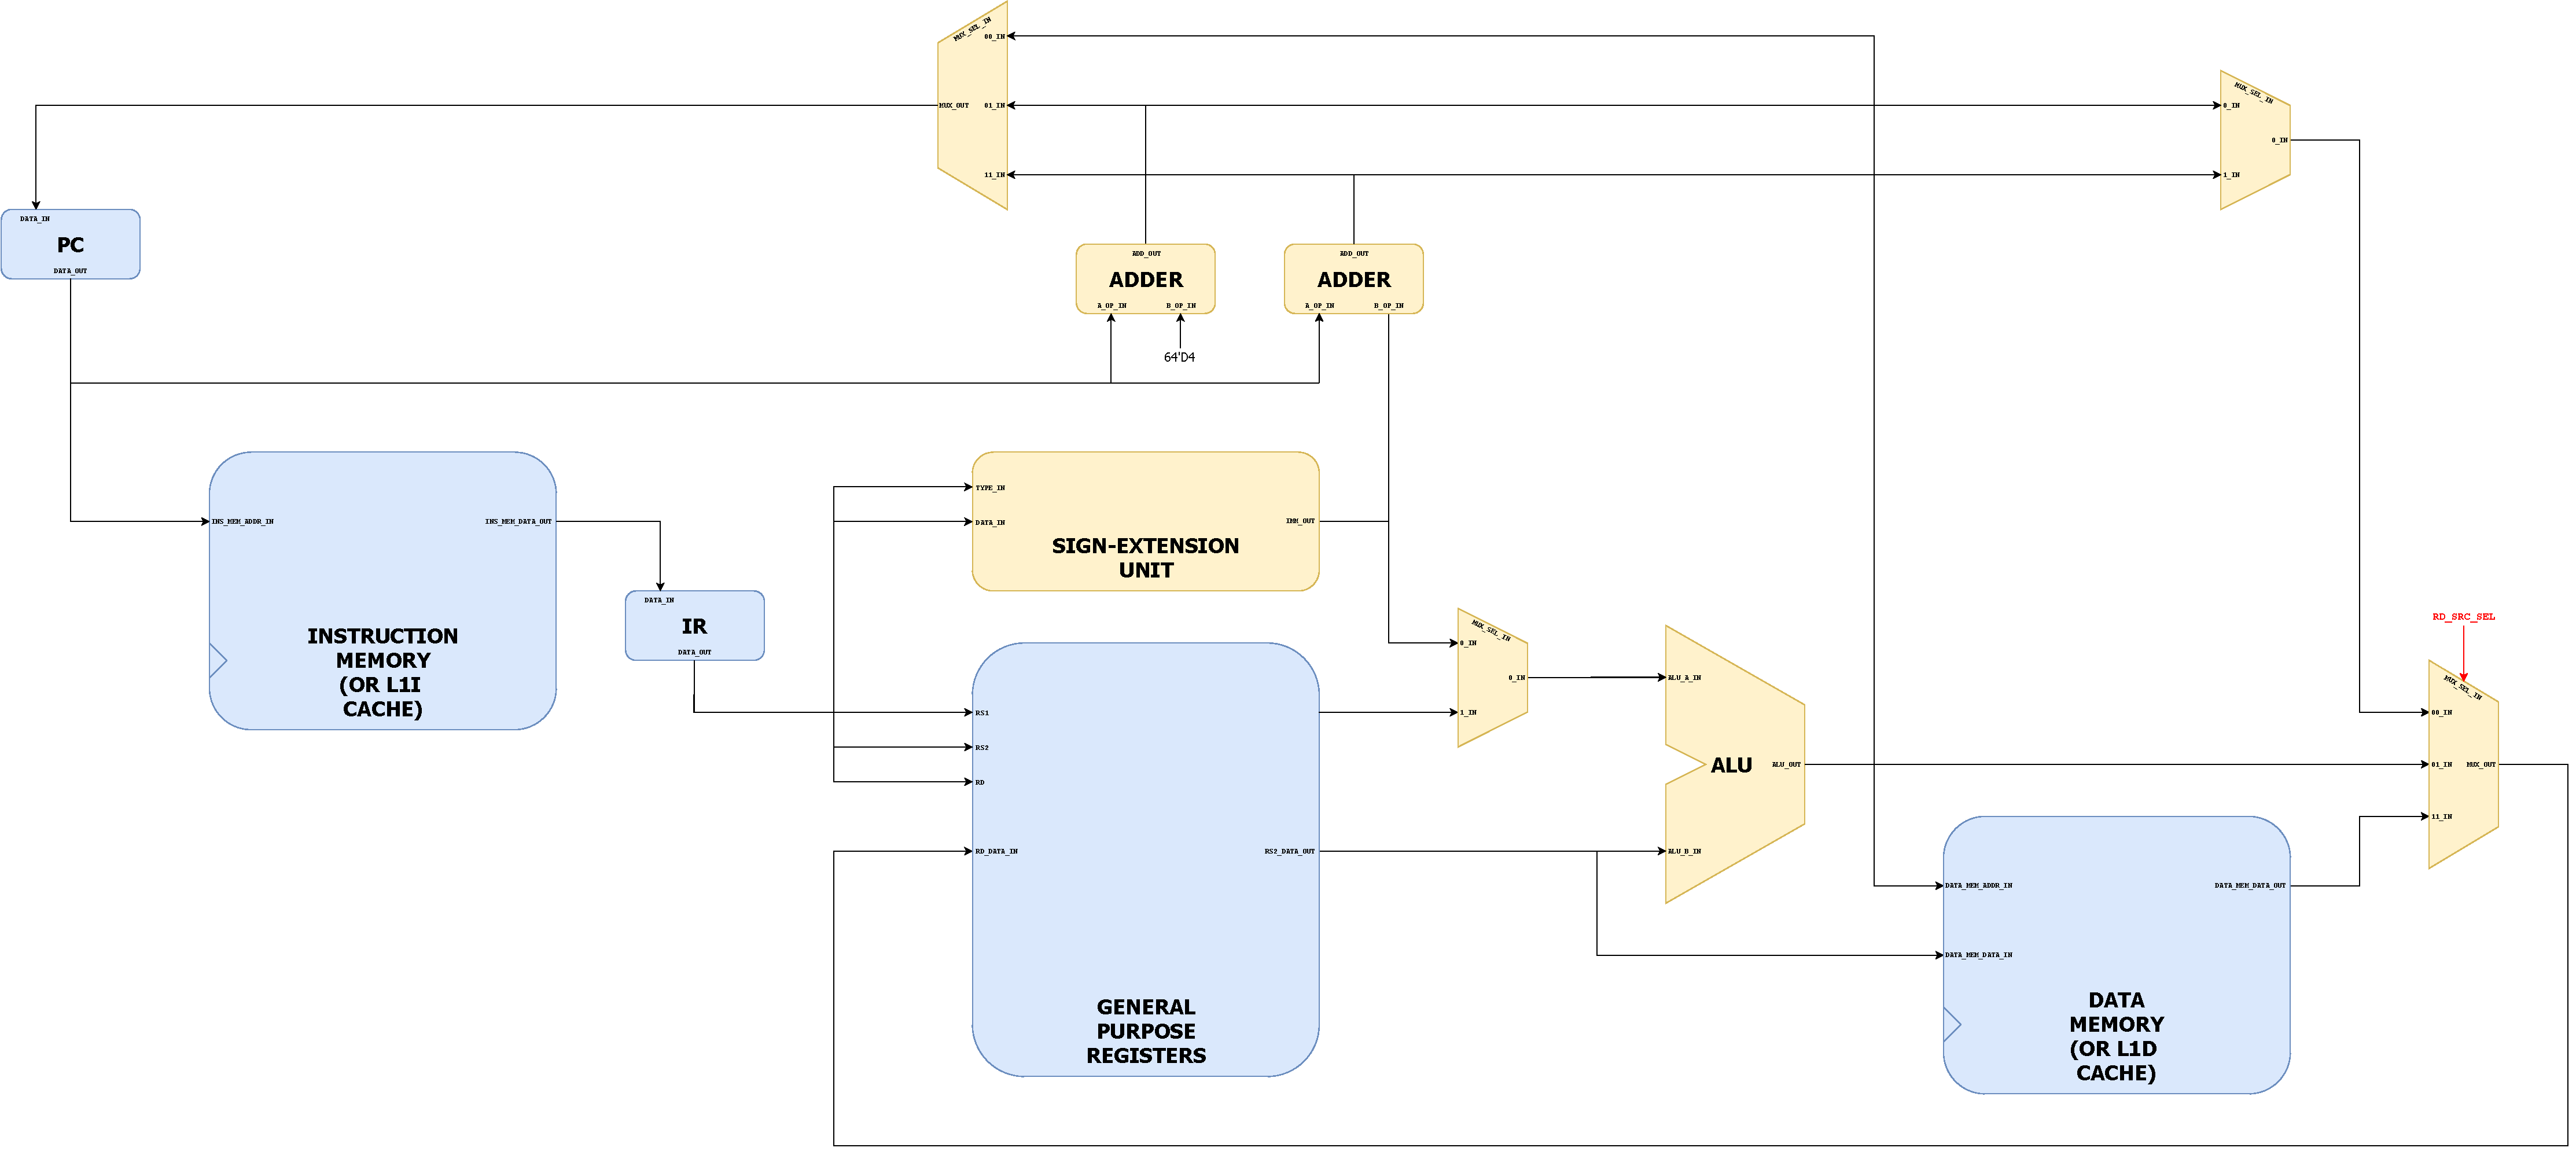
\includegraphics[width=0.95\textwidth]{resources/core101.pdf}
    \caption{Microarchitecture diagram for Core101.}
    \label{fig:uarch}
\end{figure}

\appendix
\section{Previous specifications}


\end{document}
